% Created 2022-10-12 Wed 19:34
% Intended LaTeX compiler: pdflatex
\documentclass[11pt]{article}
\usepackage[utf8]{inputenc}
\usepackage[T1]{fontenc}
\usepackage{graphicx}
\usepackage{grffile}
\usepackage{longtable}
\usepackage{wrapfig}
\usepackage{rotating}
\usepackage[normalem]{ulem}
\usepackage{amsmath}
\usepackage{textcomp}
\usepackage{amssymb}
\usepackage{capt-of}
\usepackage{hyperref}
\author{Max Jauregui}
\date{\today}
\title{Finanças pessoais 2022}
\hypersetup{
 pdfauthor={Max Jauregui},
 pdftitle={Finanças pessoais 2022},
 pdfkeywords={},
 pdfsubject={},
 pdfcreator={Emacs 27.1 (Org mode 9.3)}, 
 pdflang={Pt_Br}}
\begin{document}

\maketitle
\setcounter{tocdepth}{2}
\tableofcontents


\section{Análise mensal}
\label{sec:org42e41a2}

\subsection{Outubro}
\label{sec:org93f7bc3}

\subsubsection{Saldo anterior}
\label{sec:orgb0f3714}

O saldo anterior nas contas bancárias é R\$ \texttt{3472.72}

\subsubsection{Tabela de gastos e ingressos}
\label{sec:org230132e}

\begin{verbatim}
         Data    Descrição   Valor     Forma
0  2022-10-01      Padaria   16.63   Crédito
1  2022-10-01    Cafeteria   37.52   Crédito
2  2022-10-02  Restaurante   79.80   Crédito
3  2022-10-03      Mercado  212.80   Crédito
5  2022-10-05        Trade  109.34  Depósito
6  2022-10-06   Condomínio  432.03    Débito
4  2022-10-08  Combustível   80.00   Crédito
7  2022-10-10       Cartão  478.00    Débito
8  2022-10-11      Energia   44.14    Débito
9  2022-10-11     Internet   99.90    Débito
10 2022-10-14      Aluguel  704.00    Débito
\end{verbatim}

\subsubsection{Classificação por forma de pagamento}
\label{sec:orga40c7a8}

\textbf{Crédito:} Gastos realizados usando cartão de crédito

\textbf{Débito:} Gastos realizados via PIX, pagamento de boleto, transferência bancária ou cartão de débito.

\textbf{Depósitos:} Ingressos de fontes diversas.

\begin{verbatim}
            Valor
Forma            
Crédito    426.75
Depósito   109.34
Débito    1758.07
\end{verbatim}


\begin{center}
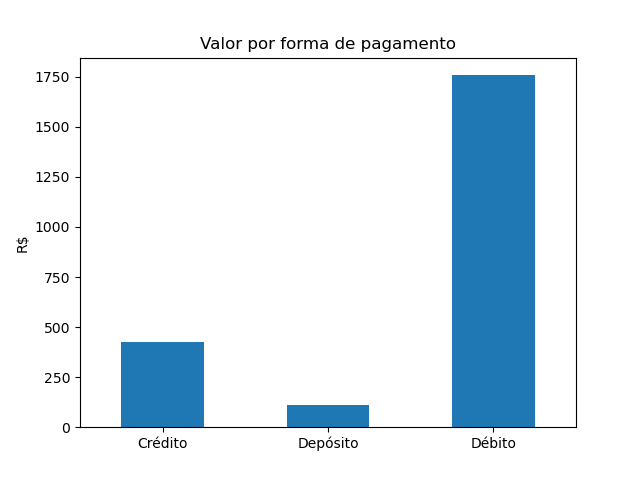
\includegraphics[width=.9\linewidth]{outubro-forma.png}
\end{center}

\subsubsection{Classificação dos gastos e ingressos}
\label{sec:org3442298}

\begin{verbatim}
                           Valor
Classe                          
Açougue/Mercado/Padaria   229.43
Fatura do cartão          478.00
Moradia                  1280.07
Renda extra               109.34
Restaurante/Cafeteria     117.32
Transporte                 80.00
\end{verbatim}


\begin{center}
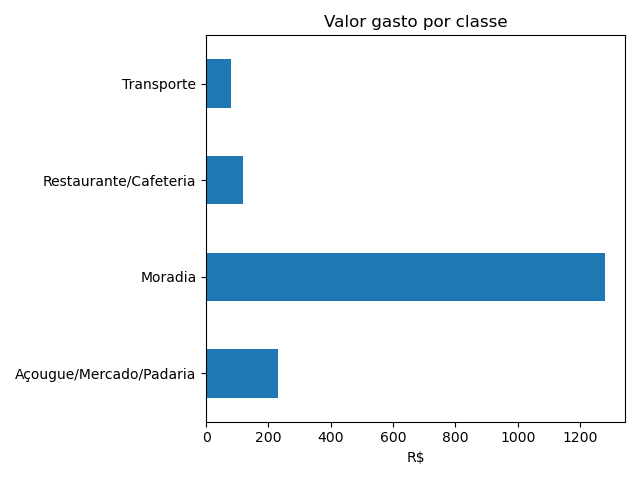
\includegraphics[width=.9\linewidth]{outubro-classe.png}
\end{center}

\subsubsection{Saldo posterior}
\label{sec:org91b37c8}

O saldo posterior nas contas bancárias é R\$ \texttt{1823.99}
\end{document}